
%----------------------------------------------------------------------------------------

\documentclass[11pt]{diazessay} % Font size (can be 10pt, 11pt or 12pt)

%----------------------------------------------------------------------------------------
%	TITLE SECTION
%----------------------------------------------------------------------------------------

\title{\textbf{Proof by Minecraft} \\ {\Large\itshape The greatest proof simulator in recorded history}} % Title and subtitle

\author{\textbf{UQCS Hackathon} \\ \textit{Pajorn, Josiah, Matt, Gus, and Zwe}} % Author and institution

\date{\today} % Date, use \date{} for no date

%----------------------------------------------------------------------------------------

\begin{document}

\maketitle % Print the title section

%----------------------------------------------------------------------------------------
%	ABSTRACT AND KEYWORDS
%----------------------------------------------------------------------------------------

%\renewcommand{\abstractname}{Summary} % Uncomment to change the name of the abstract to something else

\begin{abstract}
Minecraft is widely known as a sandbox for creativity, but we extend its potential to the domain of formal reasoning: First Order Logic (FOL) and Boolean Algebra. 
Our project, Proof by Minecraft, transforms logical expressions into interactive visual proofs. 
Using Python, we parse and simplify expressions via trees and graph theory, 
then generate corresponding Minecraft circuits. 
A Tkinter-based interface allows users to input one or two expressions; the system produces a truth table, evaluates equivalence, and constructs a Minecraft representation of the logic. This approach makes formal logic both intuitive and engaging, offering a novel way to explore proofs—because sometimes, the best argument really is Proof by Minecraft.
\end{abstract}

\hspace*{3.6mm}\textit{Keywords:} First Order Logic/Boolean Algebra (FOL), Graph Theory, Trees % Keywords

\vspace{30pt} % Vertical whitespace between the abstract and first section

%----------------------------------------------------------------------------------------
%	ESSAY BODY
%----------------------------------------------------------------------------------------

\section*{Rationale - Key Ideas, Requirements, and Goals.}
The main idea behind 'Proof by Minecraft' is to make a formal logic system which is not only rigorous but visually and interactively intuitive.
It both provides a 'graphical' representation of logical expressions, and also allows users to interact with the circuit, using levers to change the value of the inputs, and to evaluate the expression.
The system also provides definitive feedback like truth tables, and equivalences which are essential for rigorously evaluating logical expressions.
By embedding First Order Logic (FOL) expressions within Minecraft, we provide users with a tangible way to explore equivalence, simplification, and proofs. Our rationale stems from three guiding goals: accessibility, interactivity, and clarity.

\subsubsection*{Key Ideas}
\begin{itemize}
    \item Each FOL expression is represented as a Minecraft world where levers act as input variables and redstone lamps display output values.  
    \item When two expressions are entered, they are rendered side by side with shared inputs, enabling direct comparison.  
    \item To evaluate equivalence, the program systematically generates all input cases ($2^n$ possibilities) and maps them into Minecraft.  
\end{itemize}

\subsubsection*{Requirements}
\begin{itemize}
    \item \textbf{Parsing and Representation:} Logical expressions must be parsed into a graph/tree structure using graph theory and algorithmic simplification.  
    \item \textbf{User Interface:} A Python GUI (Tkinter) must allow users to input expressions, following Nielsen’s 10 heuristics for usability.  
    \item \textbf{Minecraft Integration:} The parsed structure must be translated into a Minecraft world file, ensuring correct placement of redstone, lamps, and levers.  
\end{itemize}

\subsubsection*{Goals}
\begin{itemize}
    \item Provide an engaging, gamified method to explore logical proofs.  
    \item Demonstrate how graph theory and algorithms can be applied creatively.  
    \item Produce both a truth table and equivalence check alongside the Minecraft visualization.  
\end{itemize}


%------------------------------------------------

\section*{Section Name}

\begin{wrapfigure}{l}{0.42\textwidth} % Inline image example, use an 'r' column type to position the figure on the right
	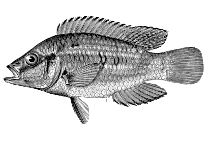
\includegraphics[width=\linewidth]{fish.png}
	\caption{An example fish.}
\end{wrapfigure}


\begin{itemize}
	\item First bullet point item
	\item Second bullet point item
	\item Third bullet point item
\end{itemize}

\begin{enumerate}
	\item First numbered list item
	\item Second numbered list item
\end{enumerate}

%------------------------------------------------

\section*{Conclusion}


%----------------------------------------------------------------------------------------
%	BIBLIOGRAPHY
%----------------------------------------------------------------------------------------

\bibliographystyle{unsrt}

\bibliography{sample.bib}

%----------------------------------------------------------------------------------------

\end{document}
